% Payung proposal to Income Insurance, Singapore-India Hackathon 2026 (FinTech track).
% Compile with: tectonic safeday-proposal.tex   (or xelatex / pdflatex twice)
% Figures live in figures/. References are numbered in order of first use.

\documentclass[11pt,a4paper]{article}

\usepackage{iftex}
\ifPDFTeX
  \usepackage[T1]{fontenc}
  \usepackage{tgheros}
  \renewcommand{\familydefault}{\sfdefault}
\else
  \usepackage{fontspec}
  \setmainfont{texgyreheros}[Extension=.otf, UprightFont=*-regular, BoldFont=*-bold,
    ItalicFont=*-italic, BoldItalicFont=*-bolditalic]
  \setsansfont{texgyreheros}[Extension=.otf, UprightFont=*-regular, BoldFont=*-bold,
    ItalicFont=*-italic, BoldItalicFont=*-bolditalic]
\fi
\usepackage[a4paper,margin=2cm]{geometry}
\usepackage{amsmath}
\usepackage{microtype}
\usepackage[dvipsnames,table]{xcolor}
\usepackage{graphicx}
\usepackage{tabularx}
\usepackage{xltabular}
\usepackage{array}
\usepackage[shortlabels]{enumitem}
\usepackage{titlesec}
\usepackage{caption}
\usepackage{float}
\usepackage{tikz}
\usetikzlibrary{arrows.meta,positioning}
\usepackage{pgfplots}
\pgfplotsset{compat=1.18}
\usepackage[most]{tcolorbox}
\usepackage{xfp}
\usepackage{siunitx}
\usepackage[super,sort&compress,comma]{natbib}
\usepackage[hidelinks]{hyperref}

\definecolor{ink}{HTML}{1F2A44}
\definecolor{accent}{HTML}{1D5FA8}
\definecolor{soft}{HTML}{EEF3FA}
\definecolor{rule}{HTML}{9AA5B8}
\definecolor{good}{HTML}{E8F4EC}
\definecolor{bad}{HTML}{FBEAEA}
\definecolor{measured}{HTML}{2E7D4F}
\definecolor{assumed}{HTML}{B35C00}

\titleformat{\section}{\Large\bfseries\color{ink}}{\thesection}{0.6em}{}
\titleformat{\subsection}{\large\bfseries\color{ink}}{\thesubsection}{0.6em}{}
\titlespacing*{\section}{0pt}{1.4em}{0.5em}
\titlespacing*{\subsection}{0pt}{1.1em}{0.4em}
\captionsetup{font=small,labelfont=bf}
\setlist{itemsep=0.35em,topsep=0.4em}
\setlength{\parindent}{0pt}
\setlength{\parskip}{0.65em}
\renewcommand{\arraystretch}{1.3}
\setlength{\extrarowheight}{2pt}
\setlength{\tabcolsep}{7pt}
\setlength{\arrayrulewidth}{0.5pt}
\arrayrulecolor{rule}
\setlength{\LTpre}{0.6em}
\setlength{\LTpost}{0.6em}
% Columns: L/C/R fixed width; Y and Z stretch. Term sheets pair a bold item (K) with sentences (Y).
\newcolumntype{L}[1]{>{\raggedright\arraybackslash}p{#1}}
\newcolumntype{C}[1]{>{\centering\arraybackslash}p{#1}}
\newcolumntype{R}[1]{>{\raggedleft\arraybackslash}p{#1}}
\newcolumntype{K}[1]{>{\bfseries\raggedright\arraybackslash}p{#1}}
\newcolumntype{Y}{>{\raggedright\arraybackslash}X}
\newcolumntype{Z}{>{\centering\arraybackslash}X}
\newcommand{\head}{\rowcolor{soft}}
\newcommand{\sgd}{\textup{S\$}}
\newcommand{\measured}{\textcolor{measured}{\textbf{Measured.}}}
\newcommand{\assumed}{\textcolor{assumed}{\textbf{Assumption.}}}
% Business case: \bizPremium is the Tier 1 cooked food yearly premium with GST at the median of the
% 103 hawker centres (/api/map/quotes, final tariff of 15 Nov 2026, run on 16 Nov 2026). Every \biz
% cell is worked out from it: \biz{share of premium without GST}{number of stalls}.
\def\bizPremium{574.92}
\newcommand{\biz}[2]{\sgd\num[group-separator={,},group-minimum-digits=4]{\fpeval{round(\bizPremium/1.09*(#1)*(#2),0)}}}
% Footnotes use symbols, so they do not look like the numbered references.
\renewcommand{\thefootnote}{\fnsymbol{footnote}}

\begin{document}

% ---------------------------------------------------------------- Title
\begin{center}
  {\bfseries\huge\color{ink} Payung}\par\vspace{0.3em}
  {\Large Weather income cover for Singapore's hawkers and small shops}\par\vspace{0.7em}
  {\small A proposal to Income Insurance \quad|\quad Singapore-India Hackathon 2026, FinTech and InsurTech track}\par\vspace{0.2em}{\small Team SIH-FIN-4}
\end{center}

\begin{tcolorbox}[colback=soft,colframe=accent,boxrule=0.6pt,arc=2pt,left=8pt,right=8pt,top=6pt,bottom=6pt]
\textbf{In short.}
\begin{itemize}[leftmargin=1.2em,itemsep=0.25em,topsep=0.25em]
  \item \textbf{The problem.} When haze, a downpour or a dangerous heat spell keeps customers away, a hawker loses the day's sales and often the day's stock. No insurance in Singapore pays for that, because existing cover pays only for physical damage.\cite{ps,mse-hawker}
  \item \textbf{The product.} Payung, offered by Income, reads NEA's public weather readings. It works out how much of a normal day's sales the weather took, and pays that share of the chosen daily amount to the stallholder's PayNow the same day. A government lockdown or closure order pays the full daily amount. There is no claim form and no loss adjuster.
  \item \textbf{The customer.} Hawkers, whose typical income is in the second-lowest income decile, and small shops.\cite{koh-hawker} A median cooked food stall pays \sgd 1,450 a month in rent.\cite{mse-rent}
  \item \textbf{The price.} Tier 1, the smallest tier, costs a cooked food stall \sgd 37.62 to \sgd 61.37 a month (\sgd 8.68 to \sgd 14.16 a week) at the 103 hawker centres, about 3\% of the median rent. That is more than the brief's ``few dollars a week''. A shop selling packaged food pays about \sgd 15 a month. The price comes from the same readings and the same rule that pay.
  \item \textbf{The tier.} We suggest the biggest tier that pays no more than the business loses on a day with no sales: Tier 1 for a stall selling \sgd 150 a day, Tier 2 at \sgd 500. Bigger tiers are not offered to it.
  \item \textbf{The value.} From weather alone, a customer who saved the premium instead would keep more at most places. The cover is worth most in a shock year: a 40-day lockdown pays a Maxwell stall 2.4 years of its Tier 1 premium. We show this plainly (Section \ref{sec:value}).
  \item \textbf{For Income.} Each premium keeps 7\% to 10\% as profit, after payouts, reinsurance and running costs. At Tier 1 that is about \biz{0.10}{1} per policy in an average year, or \biz{0.10}{5837} a year if every cooked food stall joins. Haze and lockdowns hit every customer at once, so 6\% of every premium goes to reinsurance.
\end{itemize}
\end{tcolorbox}

\subsection*{Key facts}

{\small
\begin{xltabular}{\textwidth}{|K{3.6cm}|Y|}
\hline
Who it is for & Hawker stalls and neighbourhood shops. The pilot starts with cooked food stalls in NEA hawker centres: 5,837 stalls in 103 centres.\cite{nea-hawker} Platform workers come later. \\
\hline
What they can afford & No survey yet. Tier 1 is about 3\% of a median stall's \sgd 1,450 monthly rent.\cite{mse-rent} \\
\hline
What it costs & Tier 1 cooked food cover: \sgd 49.25 a month (\sgd 11.37 a week) at Maxwell Food Centre, \sgd 37.62 to \sgd 61.37 a month across the 103 centres. \\
\hline
Which tier & The biggest tier whose daily amount is at or below what the business loses on a day with no sales: its normal weekday sales times its product share. A cooked food stall selling \sgd 500 a day gets Tier 2. \\
\hline
What it pays & A share of a chosen daily amount (\sgd 35, \sgd 195, \sgd 630 or \sgd 1,355) on each day that haze, heavy rain, heat or a flood alert hits the business. A lockdown or closure order pays the full amount. \\
\hline
How much it pays & Up to 45 full days a year in every tier, so a 40-day lockdown is paid in full: \sgd 1,575 to \sgd 60,975 a year. \\
\hline
How fast & The same evening, straight to PayNow. The customer does not need to claim. \\
\hline
What Income keeps & Everyday rain and heat payouts. 6\% of every premium is set aside to reinsure haze and lockdown years; the structure is still open. \\
\hline
What Income earns & 7\% to 10\% of premium without GST, by tier. At Tier 1 that is 10\%, about \biz{0.10}{1} per policy in an average year. \\
\hline
How it is sold & Through the customer's own Income adviser or an association. Never directly. \\
\hline
What we ask & A six-month pilot with about 300 stalls through one hawker association. \\
\hline
\end{xltabular}}

\subsection*{How this proposal answers the brief}

The problem statement asks for eight things and five must-haves.\cite{ps} Each one has its own place in this document.

{\small
\begin{xltabular}{0.9\textwidth}{|C{0.8cm}|Y|L{4.6cm}|}
\hline
\head & \textbf{The brief asks for} & \textbf{Where we answer it} \\
\hline
\endhead
1 & Concept and design & Sections \ref{sec:problem} and \ref{sec:solution} \\
\hline
2 & Target groups & Section \ref{sec:customer} \\
\hline
3 & Pricing logic & Sections \ref{sec:budget} and \ref{sec:numbers} \\
\hline
4 & Unit economics and profit for Income & Sections \ref{sec:retention} and \ref{sec:business} \\
\hline
5 & Claim parameters and exclusions & Sections \ref{sec:triggers} and \ref{sec:pays} \\
\hline
6 & Expected impact and affordability & Sections \ref{sec:customer}, \ref{sec:budget}, \ref{sec:value} and \ref{sec:impact} \\
\hline
7 & Market competitiveness & Section \ref{sec:compete} \\
\hline
8 & Distribution, and how AI and data are used & Sections \ref{sec:sold}, \ref{sec:flow} and \ref{sec:pilot}, Appendix \ref{app:params} \\
\hline
\end{xltabular}}

{\small
\begin{xltabular}{0.9\textwidth}{|C{0.8cm}|Y|L{4.6cm}|}
\hline
\head & \textbf{Must-have} & \textbf{Where we answer it} \\
\hline
\endhead
A & Offered with Income & Sections \ref{sec:sold} and \ref{sec:pilot} \\
\hline
B & Independent, verifiable data & Section \ref{sec:triggers}, Appendix \ref{app:params} \\
\hline
C & Understood in under a minute & Section \ref{sec:what} \\
\hline
D & Minimal personal data, explainable decisions & Section \ref{sec:risk} \\
\hline
E & No new hardware & Section \ref{sec:flow} \\
\hline
\end{xltabular}}

\subsection*{Words used in this proposal}

{\small
\begin{xltabular}{\textwidth}{|K{3.6cm}|Y|}
\hline
Parametric cover & Insurance that pays when a public measurement crosses a set level, instead of after an assessment of the actual loss. \\
\hline
PSI & Pollutant Standards Index. NEA's measure of haze. Above 100 is unhealthy. \\
\hline
WBGT & Wet Bulb Globe Temperature. NEA's measure of heat stress, which combines heat, humidity, sun and wind. \\
\hline
Severity & How bad a reading is, on a scale from 0\% to 100\%. \\
\hline
Hazard weight & The share of a day's sales a hazard takes away at its worst. \\
\hline
Product share & How much of that loss a stall really suffers, given what it sells. \\
\hline
Tier & The plan a customer picks. It sets the daily amount and the payout share. \\
\hline
Daily amount & What a tier pays for a day with no sales: \sgd 35, \sgd 195, \sgd 630 or \sgd 1,355. A partly bad day pays its share. \\
\hline
Loss-day & One full day's payout. A day at 24\% loss counts as 0.24 loss-days. \\
\hline
Yearly limit & The most loss-days a tier pays in any 365 days: 45 in every tier. Once it is reached, nothing more is paid until earlier payouts fall out of that window. \\
\hline
Lockdown or closure order & A government order that closes the business. It pays the full daily amount for each day. It is priced as one 40-day lockdown every 20 years. \\
\hline
Severe haze payout & An option that pays 25 times the daily amount once, when the region's PSI is above 100 on 40 or more days in a policy year. \\
\hline
Waiting period & The first 30 days of cover, and the 30 days after a move up a tier, when nothing is paid. \\
\hline
Reinsurance & Insurance that Income buys for its own book, to pay part of a year when every customer is hit at once. \\
\hline
Payout share & The share of the premium without GST that is expected to go back as payouts: 55\% to 70\%, by tier. Insurers call it the target loss ratio. \\
\hline
Cover multiple & The most a tier can pay in a year, divided by its yearly price. The quote says ``up to N times what you pay''. \\
\hline
Not offered here & A tier that cannot be bought. At a place: its price is more than half its yearly limit. For a business: it pays more than the business loses on a day with no sales. \\
\hline
Self-insure test & Whether a tier pays more than saving its premium would. It passes at a place when a 2015-type weather year pays back more than one year's premium. \\
\hline
Combined ratio & Payouts plus running costs and reinsurance, as a share of premium without GST. Below 100\% means the insurer makes a profit. \\
\hline
Back-test & Replaying past weather through today's pricing to see what the cover would have paid. \\
\hline
\end{xltabular}}

\begin{tcolorbox}[colback=white,colframe=accent,boxrule=0.6pt,arc=2pt,left=8pt,right=8pt,top=5pt,bottom=5pt,title={\bfseries A hazy week at Tekka Centre},coltitle=white,colbacktitle=accent]
A cooked food stall at Tekka Centre in Little India usually serves about 500 customers a day. In October 2026, as the haze settled over Singapore, that fell to about 200. ``Now got no business,'' the stallholder told The Straits Times.\cite{st-haze} The stall was not damaged, so its insurance paid nothing. With Payung, every unhealthy haze day would have sent money to the stall's PayNow account that evening, more on the days the PSI passed 200, with no form to fill in.
\end{tcolorbox}

% ---------------------------------------------------------------- 1
\section{The problem today}\label{sec:problem}

\subsection{Who loses money when the weather turns?}

Singapore's small traders feel the weather in their till before anyone else does. The examples below come from our team's field notes and from public reporting.

\begin{itemize}[leftmargin=1.2em]
  \item \textbf{Stalls that depend on visitors.} Singapore welcomed 16.9 million visitors in 2025.\cite{stb} Many eat at hawker centres in Chinatown, Little India and Sentosa, and on a hazy day they stay indoors. During the October 2026 haze, a Tekka Centre stall went from about 500 customers a day to about 200, and a restaurant chain saw footfall fall by roughly 40\%.\cite{st-haze}
  \item \textbf{Stalls next to offices and schools.} In a heavy downpour or a very hot afternoon, the lunch crowd orders in or eats in the canteen. The cooked food is thrown away at closing time.
  \item \textbf{Fresh food sellers.} A fishmonger or fruit seller buys stock for a few days at a time. When customers stay away, that stock spoils, which is a real cost on top of the lost sales.
  \item \textbf{Open-air and outdoor businesses.} Open-air stalls, rented sports pitches and delivery riders all lose working hours in high heat. Each hot day costs an outdoor worker a median of \sgd 21, about a quarter of the day's pay.\cite{heatsafe}
\end{itemize}

The cost adds up across the economy:
\begin{itemize}[leftmargin=1.2em]
  \item The 2026 haze cost Singapore an estimated \sgd 2.32 billion by 31 October, more than the 2015 episode after inflation.\cite{ntu-haze}
  \item Heat cut an estimated \sgd 1.18 billion of output in 2018. That figure is projected to reach \sgd 2.22 billion by 2035.\cite{heatsafe}
\end{itemize}

\subsection{Why does today's insurance not help?}

\begin{itemize}[leftmargin=1.2em]
  \item About two in three cooked food stallholders already buy stall insurance, and NEA is reviewing whether to make it compulsory.\cite{mse-hawker} That cover pays for fire, theft and damage.
  \item Even Income's SmartBiz 360 pays for business interruption only when it is caused by physical damage to the premises.\cite{ps} A hazy week breaks nothing, so there is nothing to claim.
  \item A traditional claim needs proof of lost sales and a loss adjuster. For a small stall, that costs more than the claim is worth.
\end{itemize}

\subsection{What have other countries learned?}

The problem statement lists more than a dozen schemes around the world.\cite{ps} Four of them shape Payung:

\begin{itemize}[leftmargin=1.2em]
  \item \textbf{SEWA heat cover (India) and ZhongAn's 37\,\textdegree C cover (China).} A first season with no payout destroys trust. Triggers must be set from local history, not from record extremes.
  \item \textbf{KB Insurance stallholder cover (South Korea).} No one bought it in ten months. The cover has to be cheap, simple and sold where traders already buy insurance.
  \item \textbf{BlockBima (Nairobi).} It paid on rain measured at the trader's own market, within a day, and 86\% of traders preferred it.
  \item \textbf{Flood card (Jakarta).} It used one gauge for the whole city. Residents did not see it as their own risk, and it was dropped.
\end{itemize}

% ---------------------------------------------------------------- 2
\section{Ten facts that make the case}\label{sec:facts}

\begin{tcolorbox}[breakable,colback=white,colframe=ink,boxrule=0.6pt,arc=2pt,left=6pt,right=6pt,top=4pt,bottom=4pt]
\begin{enumerate}[leftmargin=1.5em,itemsep=0.4em]
  \item \textbf{Haze came back hard.} From 2016 to 2025 the 24-hour PSI was unhealthy (above 100) on 0 to 6 days a year. In 2026 it was unhealthy on 39 days, including 23 days in a row from 3 to 25 October, with a peak of 230.\cite{team-data}
  \item \textbf{The 2026 haze cost \sgd 2.32 billion}, more than 2015.\cite{ntu-haze}
  \item \textbf{Haze hits everyone at once.} On an unhealthy day, on average 3.5 of Singapore's 5 regions were above PSI 100.\cite{team-data}
  \item \textbf{Heat is now routine.} WBGT reached 32\,\textdegree C on 22\% of days at a typical NEA station from January 2025 to November 2026.\cite{team-data} That is the level at which MOM requires rest breaks for heavy outdoor work.\cite{mom} 2025 had 29 days at 33\,\textdegree C or more.\cite{mss-2025}
  \item \textbf{Heavy rain is local.} An hour of 20\,mm or more fell somewhere in Singapore on 39\% of working days from 2016 to 2026. But on a typical such day, only 13\% of gauges saw it.\cite{team-data}
  \item \textbf{Records keep falling.} March 2025 was Singapore's wettest March on record. June and November 2025 were the hottest since 1929.\cite{mss-2025}
  \item \textbf{Very hot days will multiply.} Days above 35\,\textdegree C averaged 21.4 a year over the past 40 years. By 2100 they are projected at 41 to 351 a year.\cite{v3}
  \item \textbf{Rain will get more extreme.} Extreme daily rainfall is projected to rise in every season, by up to 92\% in the April to May inter-monsoon.\cite{v3}
  \item \textbf{The sea is rising.} Mean sea level could rise by up to 1.15\,m by 2100, and about 30\% of Singapore's land lies less than 5\,m above it.\cite{v3,nccs}
  \item \textbf{The gap is real.} No product in Singapore pays weather income loss to households, workers or small traders.\cite{ps}
\end{enumerate}
\end{tcolorbox}

\begin{figure}[H]
\centering
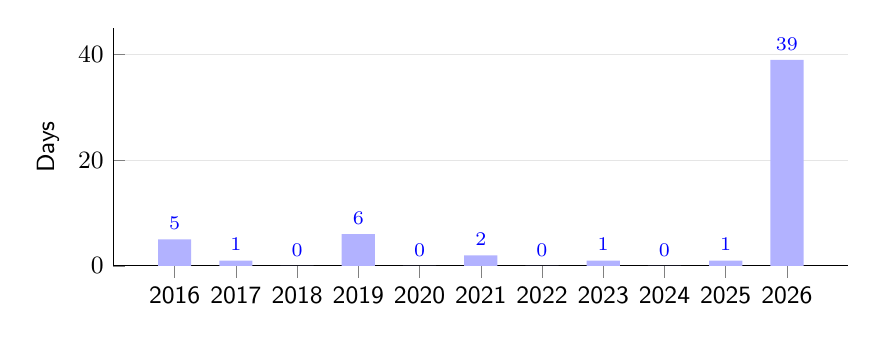
\begin{tikzpicture}
\begin{axis}[
  width=0.9\textwidth, height=4.6cm, ybar, bar width=12pt,
  symbolic x coords={2016,2017,2018,2019,2020,2021,2022,2023,2024,2025,2026},
  xtick=data, ymin=0, ymax=45, ylabel={Days}, ylabel style={font=\small},
  tick label style={font=\small}, nodes near coords, nodes near coords style={font=\scriptsize},
  axis lines*=left, ymajorgrids, grid style={draw=black!10},
  every axis plot/.append style={fill=accent!75, draw=none}]
\addplot coordinates {(2016,5) (2017,1) (2018,0) (2019,6) (2020,0) (2021,2) (2022,0) (2023,1) (2024,0) (2025,1) (2026,39)};
\end{axis}
\end{tikzpicture}
\caption{Days a year when the 24-hour PSI was unhealthy (above 100) in at least one region. Source: NEA 24-hour PSI on data.gov.sg, 9 Mar 2016 to 7 Nov 2026; 2016 and 2026 are part years.\cite{team-data}}
\end{figure}

% ---------------------------------------------------------------- 3
\section{Rare does not mean never}

People often say that Singapore is safe from extreme weather. History says otherwise, and the cost of being unprepared falls hardest on small businesses.

\begin{itemize}[leftmargin=1.2em]
  \item \textbf{A storm that was not supposed to happen.} Tropical cyclones were thought unable to form this close to the equator. In December 2001, Typhoon Vamei formed at about 1.5\,\textdegree N, just east of Singapore, the closest to the equator ever recorded.\cite{vamei} Surface winds over Singapore are projected to grow up to 20\% stronger by 2100.\cite{v3}
  \item \textbf{The wall that everyone laughed at.} In the 1970s, the mayor of Fudai, a fishing village in Japan, insisted on a 15.5\,m floodgate. Many called it a waste of money. In March 2011 a tsunami of around 20\,m reached the gate, and the village behind it was almost untouched.\cite{fudai}
  \item \textbf{When the money arrives too late.} The 2015 Chennai floods caused about US\$2.2 billion of losses, of which only US\$755 million was insured.\cite{chennai} More than 10,000 small businesses were hit, and many took months to recover because cash did not reach them quickly.\cite{mercy}
\end{itemize}

Preparing for the rare event is what protection means. A payout that arrives the same evening keeps a stall open.

% ---------------------------------------------------------------- 4
\section{Our solution: Payung}\label{sec:solution}

\subsection{What is Payung?}\label{sec:what}

Payung pays a hawker or a small shop when the weather, or a government order, takes the day's sales. It reads NEA's public readings near the business, works out how much of a normal day's sales were lost, and pays that share of a chosen daily amount to PayNow the same evening. The whole policy fits in one SMS, in English, Chinese, Malay or Tamil. This is the message for a cooked food stall at Maxwell Food Centre on Tier 1:

\begin{tcolorbox}[colback=soft,colframe=soft,arc=2pt,left=8pt,right=8pt,top=4pt,bottom=4pt]
\itshape ``Payung Tier 1: \sgd 49.25 a month, about \sgd 1.62 a day. When NEA's readings near your stall show haze, heavy rain, dangerous heat or a PUB flood alert, or a government order closes your stall, we pay up to \sgd 35 that day to your PayNow, for up to 45 full days a year. If the readings stay below the levels, nothing is paid, even if your sales were low.''
\end{tcolorbox}

The last sentence is required by the problem statement and keeps the product honest.\cite{ps}

\textbf{How the rest of this section is ordered.} Income's product lead told us how Income designs a product: start with the target customer and what they can afford, then the premium, the cover, the benefits, what Income keeps and what it reinsures, and how it is sold.\cite{income-qa} Sections \ref{sec:customer} to \ref{sec:sold} follow that order. After the benefits, Section \ref{sec:value} asks whether they are worth more than saving the premium. The price build-up comes last, in Section \ref{sec:numbers}, because it only turns those choices into a number.

Every price in this proposal comes from the platform's pricing engine with the final tariff of 15 November 2026. Maxwell Food Centre (Kim Hua Market) is our worked example. ``The median centre'' means the middle of the 103 hawker centres' prices.

% ---------------------------------------------------------------- 4a
\subsection{Who is it for, and what can they afford?}\label{sec:customer}

\textbf{The first customers} are hawker stalls and neighbourhood shops. The pilot sells to these two only.
\begin{itemize}[leftmargin=1.2em]
  \item \textbf{Hawker stalls:} 5,837 cooked food stalls in 103 NEA hawker centres, where the need and the data are clearest.\cite{nea-hawker} A typical hawker's income is in the second-lowest income decile, and the median hawker is 60 years old.\cite{koh-hawker} About two in three cooked food stallholders already buy stall insurance, which pays for fire, theft and damage.\cite{mse-hawker}
  \item \textbf{Neighbourhood shops,} such as provision shops and stalls selling packaged food. A NEA licence or UEN proves that the business trades, and so proves insurable interest. Business types follow the government's SSIC classification, which keeps sign-up clean and makes false declarations easy to spot.
  \item \textbf{Later:} Singapore's 71,600 regular platform workers, in a second phase.\cite{ps}
\end{itemize}

\textbf{What do they earn and spend?} We looked for public figures on what a hawker earns, pays and takes in.

{\small
\begin{xltabular}{\textwidth}{|K{3.2cm}|Y|}
\hline
\head What we looked for & \textbf{What we found} \\
\hline
\endhead
Hawker income & ``The income of a typical hawker has remained lower than the average Singaporean'', and in 2022 it ``corresponds to around the second lowest income decile''. To earn the \sgd 5,000 median income at \sgd 1 profit a meal, a hawker would need to sell about 200 meals a day, six days a week. Most sell fewer.\cite{koh-hawker} We found no official figure in dollars. \\
\hline
Stall rent & The median monthly rent of a non-subsidised cooked food stall was \sgd 1,450 in 2025, and \sgd 1,700 at centres run by socially-conscious enterprises.\cite{mse-rent} The older figure of about \sgd 1,250, quoted in November 2024 for the previous ten years, is out of date.\cite{koh-hawker} \\
\hline
Other monthly charges & Service and conservancy charges of about \sgd 200 and table cleaning of about \sgd 520, at the same centres, in 2025.\cite{mse-rent} With rent, that is about \sgd 2,170 a month. \\
\hline
Operating costs & Food ingredients are nearly 60\% of a stall's operating costs, manpower about 20\%, and rent less than 10\% (NEA survey, 2023).\cite{koh-hawker} So a stall paying the median rent spends more than about \sgd 14,500 a month to run. \\
\hline
Daily takings & No official figure found. From the row above, a stall that covers its costs takes in more than about \sgd 560 a day, over 26 trading days a month. This is our own rough reading, not a measured figure. \\
\hline
Platform workers & Median monthly earnings of about \sgd 1,500 to \sgd 2,500 in 2023.\cite{mom-platform} \\
\hline
The brief's target & ``A few dollars a week or month''. The Asia-Pacific average microinsurance premium is about US\$13 a year.\cite{ps} \\
\hline
What stall cover costs today & Income's Stallholder Insurance starts at \sgd 0.30 a day.\cite{income-stall} \\
\hline
\end{xltabular}}

\textbf{What share is each tier?} Each tier's monthly price for a cooked food stall at the median centre, set against those figures:

\begin{center}
\small
\begin{tabularx}{\textwidth}{|L{5.0cm}|Z|Z|Z|Z|}
\hline
\head & \textbf{Tier 1} & \textbf{Tier 2} & \textbf{Tier 3} & \textbf{Tier 4} \\
\hline
Monthly price, median centre & \sgd 47.91 & \sgd 244.68 & \sgd 729.71 & \sgd 1,457.35 \\
\hline
Share of the \sgd 1,450 median rent & 3.3\% & 16.9\% & 50.3\% & 100.5\% \\
\hline
Share of rent and charges, \sgd 2,170 & 2.2\% & 11.3\% & 33.6\% & 67.2\% \\
\hline
Share of a \sgd 5,000 income & 1.0\% & 4.9\% & 14.6\% & 29.1\% \\
\hline
Paid for a day with no sales & \sgd 35 & \sgd 195 & \sgd 630 & \sgd 1,355 \\
\hline
\end{tabularx}
\end{center}

\begin{itemize}[leftmargin=1.2em]
  \item \textbf{Tier 1 costs about 3\% of a median month's rent.} A typical hawker earns less than \sgd 5,000, so Tier 1 is more than 1\% of a typical hawker's income.
  \item \textbf{Tier 2 costs about a sixth of the rent,} and Tiers 3 and 4 half to all of it.
  \item \textbf{We have not asked stallholders what they will pay.} No survey has been done. The pilot must test it.
\end{itemize}

\textbf{Which tier does a business get?} Rent tells us what a stall can afford, but not how much cover it needs. So the tier follows what a bad day costs the business.
\begin{itemize}[leftmargin=1.2em]
  \item The sign-up asks for the business's normal sales on a weekday. A day with no sales costs the business those sales times its product share (Section \ref{sec:pays}): 1.00 for cooked food, about 0.11 for packaged food.
  \item We suggest the biggest tier whose daily amount is at or below that loss. A bigger tier is not offered, because cover must not pay more than the loss. This is insurable interest.
  \item A business that loses less than \sgd 35 on a day with no sales is not offered Payung. For a shop selling packaged food, that is normal sales below about \sgd 313 a day.
  \item Rent is shown for information only. It does not choose the tier.
\end{itemize}

\begin{center}
\small
\begin{tabularx}{\textwidth}{|Y|R{2.2cm}|R{2.4cm}|C{1.9cm}|C{2.2cm}|}
\hline
\head \textbf{Business} & \textbf{Normal weekday sales} & \textbf{Lost on a day with no sales} & \textbf{Suggested tier} & \textbf{Tiers offered} \\
\hline
Drinks stall, Maxwell Food Centre & \sgd 150 & \sgd 150 & Tier 1 & 1 \\
\hline
Chicken rice stall, Maxwell Food Centre & \sgd 500 & \sgd 500 & Tier 2 & 1 and 2 \\
\hline
Busy cooked food stall, Maxwell Food Centre & \sgd 1,500 & \sgd 1,500 & Tier 4 & 1 to 4 \\
\hline
Provision shop, postcode 380123, packaged food & \sgd 2,000 & about \sgd 224 & Tier 2 & 1 and 2 \\
\hline
\end{tabularx}
\end{center}

The three Maxwell stalls are priced as cooked food. Without the sales, as on the risk atlas, every tier the place allows is shown and none is suggested.

% ---------------------------------------------------------------- 4b
\subsection{What premium fits that budget?}\label{sec:budget}

We work backwards. What a bad day costs the business sets the biggest tier it can buy. The budget then decides whether it takes that tier or a smaller one. The premium for a given place rises in step with the daily amount, so the budget fixes the daily cover.

\begin{center}
\small
\begin{tabularx}{\textwidth}{|L{4.8cm}|Z|Z|Z|Z|}
\hline
\head \textbf{Cooked food, Maxwell Food Centre} & \textbf{Tier 1} & \textbf{Tier 2} & \textbf{Tier 3} & \textbf{Tier 4} \\
\hline
Monthly price & \sgd 49.25 & \sgd 251.54 & \sgd 750.14 & \sgd 1,498.16 \\
\hline
Weekly price & \sgd 11.37 & \sgd 58.05 & \sgd 173.11 & \sgd 345.73 \\
\hline
Price per day & \sgd 1.62 & \sgd 8.27 & \sgd 24.66 & \sgd 49.25 \\
\hline
Suggested when a day with no sales costs & \sgd 35 to under \sgd 195 & \sgd 195 to under \sgd 630 & \sgd 630 to under \sgd 1,355 & \sgd 1,355 or more \\
\hline
\end{tabularx}
\end{center}

\begin{itemize}[leftmargin=1.2em]
  \item \textbf{For a shop selling packaged food, Tier 1 meets the brief.} At postcode 380123 it costs \sgd 15.32 a month, or \sgd 3.53 a week. Packaged food keeps, so a bad day costs the shop less, and the price is lower.
  \item \textbf{For a cooked food stall, Tier 1 is above ``a few dollars a week''.} It costs \sgd 11.37 a week at Maxwell, and \sgd 8.68 to \sgd 14.16 a week across the 103 centres (median \sgd 11.06). Cooked food loses the whole day's sales, and the price carries the 2015 and 2026 haze years and the lockdown cover.
  \item \textbf{What a few dollars would buy.} At Maxwell, \sgd 3 a week buys about \sgd 9.23 of cooked food cover a day. That is about a sixth of a day's median rent (\sgd 1,450 over 26 trading days is \sgd 55.77). Tier 1's \sgd 35 is about 63\% of it.
  \item \textbf{The lockdown cover is part of every price.} It adds \sgd 138.73 a year, or \sgd 2.67 a week, to Tier 1. At Maxwell that is 23\% of the Tier 1 price.
\end{itemize}

If the pilot shows Tier 1 is too dear for hawkers, Income has three levers: a lower selling cost through an association's group scheme, a lower daily amount, or the lockdown cover as an option. Each would lower the price. None is decided.

% ---------------------------------------------------------------- 4c
\subsection{What does it cover?}\label{sec:triggers}

Every reading is public, independent and published in real time, as the problem statement requires. Appendix \ref{app:params} gives the source of each one.

{\small
\begin{xltabular}{\textwidth}{|K{2.8cm}|Y|}
\hline
Haze & We read NEA's 24-hour PSI for the stall's region. Payouts start at PSI 101, and step up at 201 and 301. These are NEA's own unhealthy, very unhealthy and hazardous bands. \\
\hline
Heavy rain & We read the wettest hour of the working day at the 3 rain gauges nearest the stall, and take the middle value. Payouts start at 20\,mm in an hour, and step up at 30 and 50\,mm. \\
\hline
Heat & We count the working hours when WBGT at the nearest NEA station is 32\,\textdegree C or more, the level at which MOM requires rest breaks. Payouts start at 2 hours, and step up at 4 and 6 hours. Stations S142 and S128 are on hold until NEA confirms their readings, so stalls near them read the next nearest station. \\
\hline
Flash flood & A PUB flood alert near the stall, active during trading hours. \\
\hline
Lockdown or closure order & A government order that closes the business for the day. It pays the full daily amount, for every product. \\
\hline
\end{xltabular}}

\textbf{How much cover in a year?} Every tier pays up to 45 full days a year. So a 40-day lockdown or closure order is paid in full. The worst year we replayed at any centre came to 14.9 full days, in 2026. A year like 2015, with an average year of rain and heat added, comes to about 16.5 full days at Maxwell, and at most 18.9 at any centre (Jurong West Street 52 Blk 505). So the limit does not run out in a haze year.

\textbf{When does cover start?} After a 30-day waiting period. A move up to a higher tier starts a new 30-day wait for the whole cover, so nobody moves up when a bad day is forecast. A move down keeps the start date.

\textbf{What does Payung not pay?}\label{sec:exclusions}
\begin{itemize}[leftmargin=1.2em]
  \item \textbf{No trigger, no payout.} If the readings stay below the levels, nothing is paid, even if sales were low. This is stated at sign-up and in every SMS.
  \item \textbf{No medical costs, injury or property damage.} Other insurance covers these, including Income's own stall and SmartBiz 360 policies.
  \item \textbf{One payout per day,} and never more than 45 full days in any 365 days. The limit counts every payout to the customer in that time, from any earlier cover.
  \item \textbf{Trading businesses only.} The business must hold a valid NEA licence or UEN on the day.
  \item \textbf{Nothing in the first 30 days,} or in the 30 days after a move up a tier.
  \item \textbf{No buying only the bad weeks.} Cover runs for a 12 or 24 month term. The severe haze payout cannot be added from May to October, when haze comes. We also propose that sign-ups pause while an NEA haze advisory or heavy rain warning is in force. The platform does not do this yet.
  \item \textbf{Payouts go only to the PayNow account linked to the customer's NRIC.} Every payout keeps a copy of the readings used.
  \item \textbf{Disputes.} A customer who questions a result gets a review of those readings. An unresolved complaint can go to FIDReC, Singapore's independent dispute centre.
\end{itemize}

% ---------------------------------------------------------------- 4d
\subsection{What does it pay?}\label{sec:pays}

{\small
\begin{center}
\begin{tabularx}{\textwidth}{|L{5.0cm}|Z|Z|Z|Z|}
\hline
\head & \textbf{Tier 1} & \textbf{Tier 2} & \textbf{Tier 3} & \textbf{Tier 4} \\
\hline
Paid for a day with no sales & \sgd 35 & \sgd 195 & \sgd 630 & \sgd 1,355 \\
\hline
Paid on a 24\% haze day (PSI 101 to 200, cooked food) & \sgd 8.40 & \sgd 46.80 & \sgd 151.20 & \sgd 325.20 \\
\hline
Yearly limit & 45 days & 45 days & 45 days & 45 days \\
\hline
Most paid in a year & \sgd 1,575 & \sgd 8,775 & \sgd 28,350 & \sgd 60,975 \\
\hline
Paid for a 40-day lockdown & \sgd 1,400 & \sgd 7,800 & \sgd 25,200 & \sgd 54,200 \\
\hline
Severe haze payout, if added & \sgd 875 & \sgd 4,875 & \sgd 15,750 & \sgd 33,875 \\
\hline
\end{tabularx}
\end{center}}

\textbf{A partly bad day pays its share.} Most bad days are not total losses. Payung works out what share of the day's sales the weather took, and pays that share of the daily amount.

\textbf{Step 1: how bad was the weather?} Each reading is matched to a step on a simple scale. For haze, NEA's own PSI bands are used:

\begin{center}
\small
\begin{tabular}{|l|c|c|c|c|}
\hline
\head \textbf{24-hour PSI} & \textbf{up to 100} & \textbf{101 to 200} & \textbf{201 to 300} & \textbf{above 300} \\
\hline
How bad (severity) & 0\% & 30\% & 60\% & 100\% \\
\hline
\end{tabular}
\end{center}

Rain and heat use the same 30\%, 60\% and 100\% steps, at the levels in Section \ref{sec:triggers}.

\textbf{Step 2: how much of the day's sales does that take?}
\begin{center}
\fbox{\parbox{0.85\textwidth}{\centering\vspace{2pt}
Loss from one hazard \;=\; weight \;$\times$\; severity \;$\times$\; product share\vspace{2pt}}}
\end{center}
\begin{itemize}[leftmargin=1.2em]
  \item The \textbf{weight} is the share of sales a hazard takes at its worst: 80\% for haze, 50\% for heavy rain and 40\% for heat. A closure order counts as a full day lost.
  \item These are starting values that real data can test. At PSI 201 to 300, the haze weight gives a 48\% loss for a cooked food stall. Stalls reported falls of 20\% to 60\% in October 2026.\cite{st-haze}
  \item The \textbf{product share} adjusts for what the stall sells (see below).
\end{itemize}

\textbf{Step 3: put the hazards together.} If haze and rain hit on the same day, they are not simply added, because the total can never pass 100\%:
\begin{center}
\fbox{\parbox{0.85\textwidth}{\centering\vspace{2pt}
Day's loss \;=\; 1 \;$-$\; (1 $-$ haze loss) $\times$ (1 $-$ rain loss) $\times$ (1 $-$ heat loss)\vspace{2pt}}}
\end{center}

\textbf{Step 4: pay.} \quad Payout \;=\; day's loss \;$\times$\; the tier's daily amount.

\textbf{A worked example.} A day with PSI 230 (severity 60\%) and a 35\,mm rain hour (severity 60\%), on Tier 1 (\sgd 35 a day):

\begin{center}
\small
\begin{tabular}{|l|c|c|}
\hline
\head & \textbf{Cooked food stall} & \textbf{Fresh produce stall} \\
\hline
Haze loss & 80\% $\times$ 60\% $\times$ 1.00 = 48.0\% & 80\% $\times$ 60\% $\times$ 0.35 = 16.7\% \\
\hline
Rain loss & 50\% $\times$ 60\% $\times$ 1.00 = 30.0\% & 50\% $\times$ 60\% $\times$ 0.35 = 10.4\% \\
\hline
Day's loss & 1 $-$ 0.52 $\times$ 0.70 = 63.6\% & 1 $-$ 0.833 $\times$ 0.896 = 25.4\% \\
\hline
\textbf{Payout} & \textbf{\sgd 22.26} & \textbf{\sgd 8.89} \\
\hline
\end{tabular}
\end{center}

\textbf{Why does the product matter?} Stock is inventory, not equipment. A bad day costs a stall two things:
\begin{itemize}[leftmargin=1.2em]
  \item \textbf{the profit on sales that never come back,} which is how insurers measure lost income;\cite{marsh}
  \item \textbf{the stock that spoils} before it can be sold, which insurers usually cover separately.\cite{zurich}
\end{itemize}
The stall and its equipment are already covered by property insurance, so Payung leaves them out.
\begin{center}
\fbox{\parbox{0.85\textwidth}{\centering\vspace{2pt}
Product share \;=\; share of demand lost \;$\times$\; ( lost profit \;+\; cost of spoiled stock )\vspace{2pt}}}
\end{center}
Profit margins come from Singapore's Annual Survey of Services 2024. Food and beverage outlets spend 32.9\% of their revenue on goods, and retail shops spend 68.0\%.\cite{singstat}

{\small
\begin{xltabular}{\textwidth}{|K{3.6cm}|C{1.6cm}|Y|}
\hline
\head What the stall sells & \textbf{Share} & \textbf{Why} \\
\hline
\endhead
Cooked food & 1.00 & Unsold food is thrown away at closing time, and a missed meal is not bought later. \\
\hline
Flowers & 0.45 & Most of the stock wilts before the next sale. \\
\hline
Fresh produce & 0.35 & Some stock spoils, but some can still be sold the next day. \\
\hline
Packaged food and general goods & 0.11 & The stock keeps, so only part of the profit on lost sales is gone. \\
\hline
\end{xltabular}}

\textbf{Lockdown and closure orders pay in full.} A government order that closes the business pays the full daily amount for every day it lasts, up to 45 days a year, whatever the business sells. There is no history to price it from, so we assume one 40-day lockdown or closure order every 20 years: 2 days a year. This is a team assumption until Income gives its view.

\textbf{The severe haze payout} is an option on top of any tier. If the region's 24-hour PSI is 101 or more on 40 or more days in a policy year, it pays 25 times the daily amount, once. It costs a tenth of that payout a year: \sgd 87.50 a year (\sgd 1.68 a week) on Tier 1, for a \sgd 875 payout. That price assumes a 5.5\% chance a year, about 1 year in 18, with 60\% of the price going back as payouts. Since April 2014, only 2015 reached 40 days, in 3 of the 5 regions. 2026 did not. The chance is a team assumption until a longer haze record is checked. The option cannot be added from May to October, and it has its own 30-day wait.

\textbf{What would it have paid?} Every quote shows these numbers for each tier. Each one is a replay of real days at the customer's own place, with that tier. None of them is a promise.

{\small
\begin{xltabular}{\textwidth}{|K{4.4cm}|Y|}
\hline
\head The quote says & \textbf{How it is worked out} \\
\hline
\endhead
Monthly price, then weekly and daily & The yearly price divided by 12, 52 and 365. The premium is collected weekly. \\
\hline
Up to N times what you pay & The most the tier pays in a year, divided by its yearly price. \\
\hline
A typical year paid & The middle yearly payout, 2017 to 2025, and the average number of days with any payout. \\
\hline
Paid in X of the last N years & The years from 2017 to 2026 with at least one payout. \\
\hline
In 2026 & What the tier would have paid in 2026, to the last day of data. \\
\hline
A year like 2015 & The 2015 haze loss-days plus an average year's rain and heat loss-days, capped at the yearly limit, times the daily amount. Weather only: no lockdown. \\
\hline
In a 40-day lockdown & 40 days times the daily amount. \\
\hline
Priced to return & Expected payouts divided by the price with GST: about 50\% to 64\%, by tier. \\
\hline
Best value & The tier with the highest multiple that is offered at that place. \\
\hline
\end{xltabular}}

For a Tier 1 cooked food stall at Maxwell Food Centre, the quote reads:

\begin{tcolorbox}[colback=soft,colframe=soft,arc=2pt,left=8pt,right=8pt,top=4pt,bottom=4pt]
\begin{enumerate}[leftmargin=1.4em,itemsep=0.2em,topsep=0.1em]
  \item ``\sgd 49.25 a month. Up to \sgd 1,575 a year: 2.7 times what you pay.''
  \item ``A typical year paid \sgd 103, spread over about 17 days with a part payout.''
  \item ``A stall here would have been paid in each of the last 10 years.''
  \item ``In 2026, a stall here would have been paid \sgd 378 in total.''
  \item ``We estimate a year like 2015 would pay about \sgd 578. It does not run out before 45 bad days.''
  \item ``In a 40-day lockdown: \sgd 1,400.''
\end{enumerate}
\end{tcolorbox}

The 17 days are days with any payout, most of them part days. A typical year pays back much less than the price: \sgd 103 of the \sgd 591.02 a year. The price expects \sgd 298.22 of payouts a year, about half of what the customer pays. The gap has three causes. The haze years, 2015 and 2026, pay far more than a typical year. The price carries 2 lockdown days a year (\sgd 70 of payouts) that no replayed year has used. And it adds the average heat loss to the years before NEA's heat readings start in 2025. We tell the customer this plainly.

% ---------------------------------------------------------------- 4d2
\subsection{Is it worth more than saving the premium?}\label{sec:value}

Income's product lead asked: ``Pay a premium of say \$10 and my payout is \$20, would I see value, or would I rather save \$10 and self-insure?''\cite{income-qa} So we compared two customers at the same place. One buys the tier every year. The other puts the same premium aside and pays themself what the tier would have paid.

\textbf{The self-insure test.} A tier passes at a place when a 2015-type weather year pays back more than one year's premium. One year of saving is one premium. If the worst haze year on record pays less than that, a customer could pay for it from one year's savings, and the cover adds nothing for weather.

\begin{center}
\small
\begin{tabularx}{\textwidth}{|L{4.6cm}|Z|Z|Z|Z|}
\hline
\head & \multicolumn{2}{c|}{\textbf{Cooked food, Maxwell}} & \multicolumn{2}{c|}{\textbf{Packaged food, 380123}} \\
\hline
\head & \textbf{Tier 1} & \textbf{Tier 2} & \textbf{Tier 1} & \textbf{Tier 2} \\
\hline
Yearly price & \sgd 591 & \sgd 3,018 & \sgd 184 & \sgd 939 \\
\hline
A typical year paid & \sgd 103 & \sgd 576 & \sgd 11.63 & \sgd 64.81 \\
\hline
A 2015-type weather year & \sgd 578 & \sgd 3,221 & \sgd 56.54 & \sgd 315 \\
\hline
\quad as years of premium & 0.98 & 1.07 & 0.31 & 0.34 \\
\hline
A 40-day lockdown & \sgd 1,400 & \sgd 7,800 & \sgd 1,400 & \sgd 7,800 \\
\hline
\quad as years of premium & 2.4 & 2.6 & 7.6 & 8.3 \\
\hline
Self-insure test & \cellcolor{bad}fails & \cellcolor{good}passes & \cellcolor{bad}fails & \cellcolor{bad}fails \\
\hline
\end{tabularx}
\end{center}

\begin{itemize}[leftmargin=1.2em]
  \item \textbf{Across every place,} 541 of 3,680 tier and place pairs pass: 103 hawker centres and 81 postcode areas, 5 products, 4 tiers.\cite{team-data} Cooked food passes on Tier 1 at 26 of the 103 centres, on Tier 2 at 81, on Tier 3 at 84 and on Tier 4 at all 103. Flowers pass only on Tier 4, at 5 centres and 3 postcode areas. Fresh produce, packaged food and general goods pass nowhere.
  \item \textbf{In the replay years, 2017 to 2026,} no centre had a year in which cooked food Tier 1, 2 or 3 paid back more than its premium. From weather alone, a customer who saved the premium would have kept more.
  \item \textbf{Why shops fail.} The lockdown is priced at 2 full days a year for every product, because a closure stops all sales. Weather is scaled down by the product share. So for packaged food and general goods, 67\% to 80\% of the expected payout is the lockdown allowance. For a shop, Payung today is mostly lockdown cover.
  \item \textbf{What savings cannot do} is meet a shock. A 40-day lockdown pays a Maxwell stall 2.4 years of its Tier 1 premium, and the shop 7.6 years.
\end{itemize}

\textbf{Options for the team, not yet decided.} Hiding every tier that fails would take cover away from most shops, so we do not propose it. Two changes would help. First, a selling cost at the 5\% commission Income quoted,\cite{income-qa} with the saving passed to payouts (payout shares of 67\%, 70\%, 73\% and 75\%): cooked food then passes at every centre on Tiers 2 to 4, and on Tier 1 at 96 of 103. Second, the lockdown priced by product, or sold as its own line, so that a shop's weather cover is priced on its own. The tiers and shares in this proposal are unchanged.

% ---------------------------------------------------------------- 4e
\subsection{What does Income keep, and what does it reinsure?}\label{sec:retention}

Rain and heat are local. On a typical day with a 20\,mm rain hour somewhere in Singapore, only 13\% of gauges saw it.\cite{team-data} So rain and heat bring many small payouts spread over the book. Income can keep them.

Haze and lockdowns are different, because they hit every customer at once.
\begin{itemize}[leftmargin=1.2em]
  \item \textbf{Haze.} On an unhealthy haze day, on average 3.5 of Singapore's 5 regions were above PSI 100.\cite{team-data} A severe haze payout year pays every customer in the region who added it at once: \sgd 875,000 for 1,000 Tier 1 customers.
  \item \textbf{Lockdown.} A 40-day lockdown would cost \sgd 7.8 million for 1,000 Tier 2 customers. If all 5,837 cooked food stalls held Tier 1, it would cost \sgd 8.17 million, 2.7 times that book's yearly premium before GST of \sgd 3.05 million.
\end{itemize}

\textbf{The 6\% line.} Every tier puts 6\% of its premium before GST towards reinsurance. On the full Tier 1 book that is about \sgd 183,000 a year. Our assumption is that Income keeps the everyday rain and heat payouts and a normal haze year, and buys cover for the whole book's losses above a set level in a year, for haze and lockdown years. This is our assumption only. Income's product lead asked whether haze should be kept in-house, covered by an excess layer, or shared as a percentage. That question is still open, and we have no reinsurance quote.

\textbf{What happens in a bad year?} We replayed every recorded day since April 2014 at all 103 hawker centres, with the same readings and the same yearly limits as the price.\cite{team-data} Before 2017 only haze is recorded. The table shows Tier 1 payouts as a share of premium without GST, and what Income would keep per 1,000 Tier 1 cooked food stalls.\footnote{Per 1,000 stalls: each centre's stalls pay the Tier 1 price charged there, as the 5,837 stalls are spread across the 103 centres. Income keeps the premium without GST, less 6\% for reinsurance, less 29\% for running costs, less the payouts the replay makes that year. We then scale from 5,837 stalls to 1,000. No reinsurance recovery is counted, so the bad years show the loss before reinsurance pays.}

\begin{center}
\small
\begin{tabularx}{\textwidth}{|Y|C{3.4cm}|R{4.2cm}|}
\hline
\head \textbf{Year} & \textbf{Payouts as a share of premium} & \textbf{Profit per 1,000 stalls} \\
\hline
As designed & 55\% & \sgd 52,300 \\
\hline
Normal years, 2017 to 2025 & 17\% to 33\% & \sgd 166,300 to \sgd 250,100 \\
\hline
The last 10 years, 2017 to 2026, average & 29\% & \sgd 186,600 \\
\hline
\rowcolor{bad}The 2015 haze year, haze alone & 75\% & $-$\sgd 53,600 \\
\hline
\rowcolor{bad}The 2026 haze year, to 8 November & 72\% & $-$\sgd 35,600 \\
\hline
\rowcolor{bad}A 2015 haze with an average year of rain, heat and lockdown & 118\% & $-$\sgd 277,900 \\
\hline
\rowcolor{bad}A 40-day lockdown & 268\% & $-$\sgd 1,060,300 \\
\hline
\end{tabularx}
\end{center}

\begin{itemize}[leftmargin=1.2em]
  \item Normal years pay back far less than the 55\% in the price. The price is an average that includes the haze years and 2 lockdown days a year, and no replayed year had a lockdown. It also adds the average heat loss to every year before 2025; the replay pays no heat before 2025.
  \item In 2026 a Tier 1 cooked food stall at the median centre would have received about \sgd 363, against \sgd 121 in 2025. The most any centre would have paid in 2026 is \sgd 520.52, about 15 full days. No centre reached the 45-day limit.
  \item At full uptake, a year like 2026 would cost Income about \sgd 2.19 million in Tier 1 payouts before reinsurance. The data runs to 8 November 2026, so the full year could cost more.
  \item A year like 2026 turns an average normal year's profit of \sgd 211,300 per 1,000 stalls into a loss of \sgd 35,600, so it costs about 1.2 normal years of profit. A 2015-like year costs about 2.3, and a 40-day lockdown about 6. This is why haze and lockdowns need reinsurance and a yearly limit, as the problem statement advises.\cite{ps}
\end{itemize}

% ---------------------------------------------------------------- 4f
\subsection{How is the price built?}\label{sec:numbers}

Everything below is simple arithmetic on public data. No machine learning model decides a price or a payout, so anyone can check any number, as MAS's FEAT principles expect. The price follows the World Bank's method for weather index insurance: expected payouts, plus margins for uncertainty and rare years, plus running costs.\cite{worldbank} Payung works out the expected payouts with the same readings and the same rule that pay. So the price and the payout can never disagree about the weather.

\textbf{Step 1: replay every recorded day at the stall's place.} Each day is read exactly as a payout reads it: the region's PSI, the middle of the 3 nearest rain gauges, and the nearest heat station. The day's loss is then worked out as in Section \ref{sec:pays}.
\begin{itemize}[leftmargin=1.2em]
  \item \textbf{Haze from April 2014.} We use NEA's historical 24-hour PSI from April 2014, so the 2015 haze is one of the years in the price.
  \item \textbf{Rain from December 2016, heat from January 2025.} In a year before a feed started, that hazard adds its average from the years it was recorded.
  \item \textbf{Two heat stations on hold.} Station S142 recorded 120 heat trigger days in 2026, and S128 recorded 50, against about 7 at a typical station. Until NEA confirms them, stalls near them are read at the next nearest station, for both the price and the payout.
  \item \textbf{Lockdown.} 2 assumed days a year are added, as in Section \ref{sec:pays}.
\end{itemize}

\textbf{Step 2: count the paid days in each year.} A year's loss-days are the sum of its days' losses. Each year is capped at the tier's yearly limit, because Payung never pays more than that. The expected paid days are the average of the capped years:
\begin{center}
\fbox{\parbox{0.85\textwidth}{\centering\vspace{2pt}
Expected paid days \;=\; average over the years of \;min( that year's loss-days, the yearly limit )\vspace{2pt}}}
\end{center}

\textbf{Step 3: turn paid days into a price.} The expected payout is divided by the tier's payout share. GST is added on top:
\begin{center}
\fbox{\parbox{0.85\textwidth}{\centering\vspace{2pt}
Yearly price \;=\; expected paid days \;$\times$\; daily amount \;$\div$\; payout share \;$\times$\; 1.09\vspace{2pt}}}
\end{center}

For a cooked food stall at Maxwell Food Centre on Tier 1:

\begin{center}
\small
\begin{tabularx}{\textwidth}{|L{4.2cm}|Y|R{4.2cm}|}
\hline
\head \textbf{Step} & \textbf{Calculation} & \textbf{Result} \\
\hline
Expected paid days a year & every recorded day at Maxwell, each year capped at 45, plus 2 lockdown days & 8.52 days \\
\hline
Expected payout & paid days $\times$ \sgd 35 & \sgd 298.22 \\
\hline
Premium without GST & expected payout $\div$ 0.55 & \sgd 542.22 \\
\hline
Add 9\% GST & $\times$ 1.09 & \sgd 591.02 \\
\hline
\textbf{Monthly price} & yearly price $\div$ 12 & \textbf{\sgd 49.25} \\
\hline
Weekly price & yearly price $\div$ 52 & \sgd 11.37 \\
\hline
Price per day & yearly price $\div$ 365 & \sgd 1.62 \\
\hline
\end{tabularx}
\end{center}

The 8.52 days are rounded; the engine works with more decimals. They are an average over 13 years, 2014 to 2026, plus the 2 lockdown days.

\textbf{Why does location matter?}
\begin{itemize}[leftmargin=1.2em]
  \item Each stall is priced on its own stations. A Tier 1 cooked food stall pays \sgd 37.62 to \sgd 61.37 a month, depending on the centre, because its expected paid days run from 6.51 to 10.62.
  \item Within the South region, the share of days with a heavy rain hour ranges from 2.7\% to 7.4\% between gauges. Hot days range from 0\% to 34\% between heat stations.\cite{team-data}
\end{itemize}

\textbf{What is inside each premium?} Income asked to see the premium in five parts. Each tier has its own shares, set on the premium without GST. GST of 9\% is added on top.

\begin{center}
\small
\begin{tabular}{|l|c|c|c|c|}
\hline
\head \textbf{Of every \sgd 100 before GST} & \textbf{Tier 1} & \textbf{Tier 2} & \textbf{Tier 3} & \textbf{Tier 4} \\
\hline
Expected payouts to customers & 55 & 60 & 65 & 70 \\
\hline
Reinsurance for haze and lockdown years & 6 & 6 & 6 & 6 \\
\hline
Management expenses & 12 & 10 & 8 & 7 \\
\hline
Selling and distribution & 17 & 15 & 13 & 10 \\
\hline
Expected profit and risk margin & 10 & 9 & 8 & 7 \\
\hline
\textbf{Premium without GST} & \textbf{100} & \textbf{100} & \textbf{100} & \textbf{100} \\
\hline
GST, passed to IRAS & 9 & 9 & 9 & 9 \\
\hline
\end{tabular}
\end{center}

For Tier 1 at Maxwell, the \sgd 591.02 a year splits into \sgd 298.22 of expected payouts, \sgd 32.53 of reinsurance, \sgd 65.07 of management, \sgd 92.18 of selling and distribution, \sgd 54.22 of profit and risk margin, and \sgd 48.80 of GST.

\begin{itemize}[leftmargin=1.2em]
  \item \textbf{Why bigger tiers return more.} A policy's fixed costs, such as the sign-up checks, SMS, PayNow and the sales visit, do not grow with the daily amount. So a bigger tier spends a smaller share of its premium on costs, and returns a larger share as payouts. Insurers call this a size discount. At Maxwell, Tier 1 pays up to 2.7 times its price in a year, and Tier 4 up to 3.4 times.
  \item \textbf{Reinsurance stays at 6 in every tier,} because haze and lockdown risk grow with the daily amount. The fixed costs do not, so their share falls in the higher tiers.
  \item \textbf{Tier 2 keeps the loads we started with.} A 15\% load for uncertainty becomes the 9 of profit and risk margin. A 10\% load for rare events becomes the 6 of reinsurance. Running costs of 25\% split into 10 for management and 15 for selling.
  \item \textbf{These shares are our assumptions} until Income gives its own cost figures.
\end{itemize}

\textbf{When is a tier not offered?} In two cases. At a place, a tier is not offered where its yearly price is more than half its yearly limit, because there it would pay back less than twice its price even in the worst year. For a business, a tier is not offered where it pays more for a day with no sales than the business loses on one (Section \ref{sec:customer}). Either way the quote shows ``not offered here'' with the reason in plain words, and the platform refuses to sell it. No tier goes to Income's underwriter because of its price; an application goes to the underwriter only after a past decline. At the final prices, every tier is offered at all 103 centres and 81 postcode areas, for every product. The highest is Tier 1 cooked food, at 47\% of its limit.

% ---------------------------------------------------------------- 4g
\subsection{How is it sold?}\label{sec:sold}

\begin{itemize}[leftmargin=1.2em]
  \item \textbf{The customer pays,} as they already do for stall insurance.
  \item \textbf{There is no direct sale.} Income's product lead told us that selling around a customer's agent is ``an absolute no-no''.\cite{income-qa} So Payung is sold in two ways:
  \begin{itemize}[leftmargin=1.2em]
    \item by the customer's own Income adviser, as an add-on when Stallholder Insurance or SmartBiz 360 is bought or renewed;
    \item through an association, such as a hawkers' association or a merchants' association, as a group scheme. Each member still pays their own premium. This cuts selling costs and stops people buying only before bad weather.
  \end{itemize}
  The adviser or the association fills in the sign-up with the customer, and the platform records who sold it.
  \item \textbf{Commission.} The product lead quoted 5\% to 20\%. Our selling and distribution share is 10\% to 17\% of premium without GST, by tier.\cite{income-qa}
  \item \textbf{The pilot sells to hawker stalls and shops only.} Platform workers come next. See Section \ref{sec:pilot}.
  \item \textbf{Term and payment.} Cover runs for 12 or 24 months. The quote leads with the monthly price, and the premium is collected weekly by PayNow.
  \item \textbf{Renewal rules.} When the term ends, payouts stop and the customer applies again to renew. A move to a higher tier starts a new 30-day wait for the whole cover; a move to a lower tier keeps the start date. A cover bought after a lapse waits 30 days again, and the yearly limit still counts what was paid in the last 365 days. Payouts already made are never taken back. Cover should stop if the premium is not paid; the buy page says so, but the platform does not check payments after the first week yet.
  \item \textbf{Any launch discount} is printed on the premium line with an end date, because the problem statement rules out a permanent subsidy.\cite{ps}
\end{itemize}

% ---------------------------------------------------------------- business
\section{The business case for Income}\label{sec:business}

\subsection{Where does each dollar go?}

Of every \sgd 100 a customer pays, \sgd 8.26 is GST, which is passed on to IRAS. For Tier 1, the smallest tier, the remaining \sgd 91.74 is split like this:

\begin{center}
\small
\begin{tabular}{|l|r|r|}
\hline
\head \textbf{Use} & \textbf{Share before GST} & \textbf{Of each \sgd 100 paid} \\
\hline
Expected payouts to customers & 55\% & \sgd 50.46 \\
\hline
Reinsurance for haze and lockdown years & 6\% & \sgd 5.50 \\
\hline
Management: payments, data and staff & 12\% & \sgd 11.01 \\
\hline
Selling and distribution & 17\% & \sgd 15.60 \\
\hline
\textbf{Profit and risk margin for Income} & \textbf{10\%} & \textbf{\sgd 9.17} \\
\hline
\end{tabular}
\end{center}

Payouts and running costs come to 84\% of premium without GST at Tier 1, and 84\% to 87\% across the tiers. With reinsurance, the combined ratio is 90\% to 93\%. For comparison:
\begin{itemize}[leftmargin=1.2em]
  \item Singapore's general insurers averaged 49.6\% claims and 39.0\% expenses over 2021 to 2025.\cite{mas}
  \item Income's own general business averaged 52.7\% claims and 35.5\% expenses, a combined ratio of 88.2\%.\cite{mas}
  \item Payung returns 55\% to 70\% to customers, more than most general insurance. Its running costs are 17\% to 29\% by tier, well below the industry's 39.0\%, because automatic payouts remove claims handling.
\end{itemize}

\subsection{How much does Income earn in an average year?}

Tier 1 cooked food cover, one year, at the median hawker centre price. A stall with higher sales would be suggested a bigger tier, so this is the smallest book:

\begin{center}
\small
\begin{tabularx}{\textwidth}{|Y|R{1.9cm}|R{2.3cm}|R{2.5cm}|R{2.6cm}|}
\hline
\head & \textbf{Per stall} & \textbf{Pilot, 300 stalls} & \textbf{Per 1,000 stalls} & \textbf{All 5,837 stalls} \\
\hline
Premiums paid, including GST & \biz{1.09}{1} & \biz{1.09}{300} & \biz{1.09}{1000} & \biz{1.09}{5837} \\
\hline
Premiums without GST & \biz{1}{1} & \biz{1}{300} & \biz{1}{1000} & \biz{1}{5837} \\
\hline
Expected payouts (55\%) & \biz{0.55}{1} & \biz{0.55}{300} & \biz{0.55}{1000} & \biz{0.55}{5837} \\
\hline
Reinsurance (6\%) & \biz{0.06}{1} & \biz{0.06}{300} & \biz{0.06}{1000} & \biz{0.06}{5837} \\
\hline
Running costs (29\%) & \biz{0.29}{1} & \biz{0.29}{300} & \biz{0.29}{1000} & \biz{0.29}{5837} \\
\hline
\rowcolor{good}\textbf{Profit for Income (10\%)} & \textbf{\biz{0.10}{1}} & \textbf{\biz{0.10}{300}} & \textbf{\biz{0.10}{1000}} & \textbf{\biz{0.10}{5837}} \\
\hline
\end{tabularx}
\end{center}

These figures are for an average year, priced on 2014 to 2026 with 2 lockdown days a year. Normal years keep more than this, and haze and lockdown years lose money (Section \ref{sec:retention}). These figures are before tax and before investment income on premiums held. The profit is after the cost of reinsurance, which lowers the profit in normal years and the loss in a bad one.

% ---------------------------------------------------------------- wins
\section{Why Payung wins}\label{sec:wins}

\subsection{What else is on the market?}\label{sec:compete}

None of the products below pays small traders for weather income loss.

{\small
\begin{xltabular}{\textwidth}{|K{4.4cm}|Y|}
\hline
\head What is on the market & \textbf{What it pays for} \\
\hline
\endhead
Income Stallholder Insurance & Fire, theft and damage at the stall, from \sgd 0.30 a day.\cite{income-stall} Nothing for lost sales. \\
\hline
Income SmartBiz 360 & Business interruption, but only after physical damage to the premises.\cite{ps} \\
\hline
Grab driver cover & Income lost to medical leave or hospital stays.\cite{grab} Not weather. \\
\hline
Swiss Re HazeShield & Haze cover triggered by PSI, built for larger businesses, not small traders.\cite{ps} \\
\hline
Singlife rainfall travel cover & Up to \sgd 150 for rain on holiday.\cite{ps} \\
\hline
Income Droplet & Fares on rainy rides.\cite{ps} \\
\hline
\rowcolor{good}Payung & Lost sales and spoiled stock on haze, rain, heat and flood days, and lockdown or closure orders, paid to the stallholder the same day. \\
\hline
\end{xltabular}}

\subsection{Does it help, at a price people can pay?}\label{sec:impact}

\begin{itemize}[leftmargin=1.2em]
  \item \textbf{Affordable for some, not yet for all.} Tier 1 for a cooked food stall costs \sgd 8.68 to \sgd 14.16 a week, or \sgd 1.24 to \sgd 2.02 a day, depending on the centre. That is about 3\% of a median month's rent, but more than the brief's ``few dollars a week''.\cite{ps} It is several times the \sgd 0.30 a day at which stall insurance starts.\cite{income-stall} For a shop selling packaged food, Tier 1 is about \sgd 3.50 a week, within the brief. Sections \ref{sec:customer} and \ref{sec:budget} give the evidence.
  \item \textbf{Fast.} Money arrives the same evening. India's SEWA heat cover took six to eight weeks.\cite{ps}
  \item \textbf{Real protection.} A Tier 1 cooked food stall would have been paid in each of the last 10 years at every one of the 103 centres. At the median centre it would have received about \sgd 363 in the 2026 haze year, against \sgd 121 in 2025.\cite{team-data} The yearly limit does not run out in a haze year, and a 40-day lockdown is paid in full.
  \item \textbf{Honest value.} Every quote says that, on average, about 50\% to 64\% of what the customer pays comes back as payouts, by tier, and that a typical year pays back less. We make no ``pay \sgd 1, get \sgd 5 back'' claim, as MAS fair dealing expects.\cite{mas-fd} From weather alone, a customer who saved the premium would keep more at most places; the cover is worth most in a lockdown or a 2015-type year (Section \ref{sec:value}).
  \item \textbf{Understood.} The whole policy fits in one SMS in four languages. In the pilot we will ask every customer to say back what the product does, and aim for 90\% to get it right.
\end{itemize}

% ---------------------------------------------------------------- risk
\section{Risks, rules and regulation}\label{sec:risk}

\subsection{What could go wrong, and how is it controlled?}

{\small
\begin{xltabular}{\textwidth}{|K{4.4cm}|Y|}
\hline
\head Risk & \textbf{How Payung controls it} \\
\hline
\endhead
Haze or a lockdown hits every customer at once & Each policy has a yearly limit, and 6\% of every premium goes to reinsurance for the whole book. The price includes the 2015 haze and 2 lockdown days a year, and we stress-test the book on years like 2015 and 2026 and on a 40-day lockdown, because profit margins alone cannot carry a catastrophe.\cite{ilo} The reinsurance structure is still to be agreed (Section \ref{sec:retention}). \\
\hline
The weather at the stall differs from the station & Rain is the middle of the 3 nearest gauges, and the price reads the same stations, with the same rule, as the payout. Payouts come in steps, and any result can be questioned. \\
\hline
A station reads far out of line & Heat stations S142 and S128 recorded far more hot days than any other. They are on hold until NEA confirms them, and stalls near them read the next nearest station. \\
\hline
Cover that costs too much for what it can pay & A tier priced above half its yearly limit is not offered at that place. No tier is above it today. The self-insure test (Section \ref{sec:value}) shows where weather alone pays back less than saving would. \\
\hline
People buy cover only before bad weather & Cover runs for 12 or 24 months, a 30-day waiting period applies, and a move up a tier starts a new wait. The severe haze payout cannot be added from May to October. We also propose a sign-up pause during NEA advisories, not yet built. \\
\hline
False claims & A NEA licence or UEN is checked at sign-up, and PayNow is tied to the NRIC. There is one payout a day, and the readings are stored with every payout. \\
\hline
A data feed fails & We use the next nearest station, then MSS's published records. A payout may be late, but it is never skipped. \\
\hline
Few people buy, as in Korea & Payung is sold by the customer's own adviser at stall insurance renewal and through associations. Tier 1 is about 3\% of a median stall rent, but more than a few dollars a week for cooked food, so the pilot tests what stallholders will pay. \\
\hline
Customers buy more cover than their sales & A tier that pays more for a day with no sales than the business loses on one is not offered, and the platform refuses to sell it. The sales are declared by the customer; we propose that the adviser checks them at sale. \\
\hline
\end{xltabular}}

\subsection{How does Payung meet MAS's rules?}

The product is designed around MAS's five fair dealing outcomes.\cite{mas-fd}

{\small
\begin{xltabular}{\textwidth}{|K{5.4cm}|Y|}
\hline
\head MAS fair dealing outcome & \textbf{What Payung does} \\
\hline
\endhead
1. Fair dealing is central to the culture & Every tariff change is reviewed, versioned and kept, along with the readings behind every payout. \\
\hline
2. Products suit their target customers & It is sold only to licensed, trading businesses, payouts are sized to what the business sells, and no tier is offered that pays more than the business loses on a day with no sales. \\
\hline
3. Customers are served by competent people & It is sold by the customer's own Income adviser and by trained association partners, never directly. \\
\hline
4. Information is clear and accurate & One SMS states the trigger, the payout and when nothing is paid. Customers do a say-it-back check before they buy. \\
\hline
5. Complaints are handled fairly and quickly & The stored readings are reviewed first, then Income's complaints process and FIDReC apply. \\
\hline
\end{xltabular}}

\begin{itemize}[leftmargin=1.2em]
  \item \textbf{Fair prices (FEAT).} Prices use no age, gender, race or religion, and every price can be explained from public data.
  \item \textbf{Minimal personal data (PDPA).} Only the postal code, licence, product, normal weekday sales and PayNow link are collected.
\end{itemize}

% ---------------------------------------------------------------- 6
\section{How it works, end to end}\label{sec:flow}

\textbf{Where do AI and data help?}
\begin{itemize}[leftmargin=1.2em]
  \item \textbf{Forecasts warn, they never pay.} NEA and ECMWF forecasts power early warnings, and would power the proposed sales pause. In our test, a day-ahead ECMWF forecast caught only 52\% of heavy rain trigger days, and 49\% of its warnings were wrong.\cite{team-data}
  \item \textbf{Sign-up help.} A small assistant reads the stallholder's description and suggests a product type, which the stallholder confirms. Given the daily sales, it names the tier the pricing rule suggests, and never one that is not offered.
  \item \textbf{No AI decides a price or a payout.}
  \item \textbf{No new hardware.} Everything runs on NEA's existing stations, PayNow and SMS.
\end{itemize}

\begin{figure}[htbp]
\centering
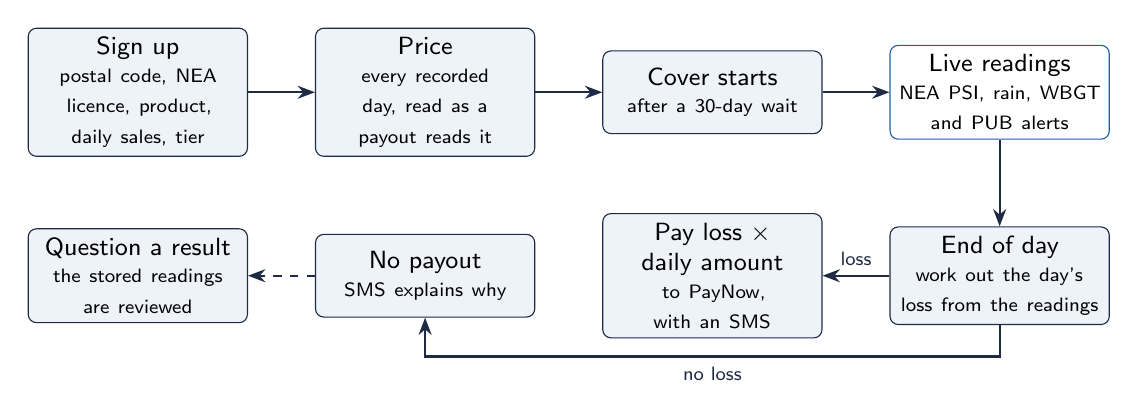
\begin{tikzpicture}[
  node distance=0.45cm and 0.85cm,
  box/.style={draw=ink, rounded corners=3pt, fill=soft, align=center, font=\small, minimum height=1.05cm, text width=2.55cm},
  data/.style={draw=accent, rounded corners=3pt, fill=white, align=center, font=\small, minimum height=1.05cm, text width=2.55cm},
  arr/.style={-{Stealth[length=2.2mm]}, thick, color=ink}]
  \node[box] (sign) {Sign up\\[-1pt]\scriptsize postal code, NEA licence, product, daily sales, tier};
  \node[box, right=of sign] (price) {Price\\[-1pt]\scriptsize every recorded day, read as a payout reads it};
  \node[box, right=of price] (start) {Cover starts\\[-1pt]\scriptsize after a 30-day wait};
  \node[data, right=of start] (feeds) {Live readings\\[-1pt]\scriptsize NEA PSI, rain, WBGT and PUB alerts};
  \node[box, below=1.1cm of feeds] (loss) {End of day\\[-1pt]\scriptsize work out the day's loss from the readings};
  \node[box, left=of loss] (pay) {Pay loss $\times$ daily amount\\[-1pt]\scriptsize to PayNow, with an SMS};
  \node[box, left=of pay] (none) {No payout\\[-1pt]\scriptsize SMS explains why};
  \node[box, left=of none] (dispute) {Question a result\\[-1pt]\scriptsize the stored readings are reviewed};
  \draw[arr] (sign) -- (price);
  \draw[arr] (price) -- (start);
  \draw[arr] (start) -- (feeds);
  \draw[arr] (feeds) -- (loss);
  \draw[arr] (loss) -- node[above, font=\scriptsize] {loss} (pay);
  \draw[arr] (loss.south) -- ++(0,-0.4) -| node[pos=0.25, below, font=\scriptsize] {no loss} (none.south);
  \draw[arr, dashed] (none) -- (dispute);
\end{tikzpicture}
\caption{The Payung workflow. Every decision stores a copy of the readings it used, so any payout can be checked later.}
\end{figure}

% ---------------------------------------------------------------- 7
\section{The working platform}

Payung already runs as a working platform on public NEA data. A stallholder signs up, checks their price and sees today's readings on a dashboard. Behind it sit two tools.

\textbf{The risk atlas.} Every NEA rain gauge and heat station is drawn as a column. The taller the column, the more often that spot has crossed the payout level in the past. Two stalls a few kilometres apart can face very different weather, which is why Payung prices by place.

\begin{figure}[htbp]
\centering
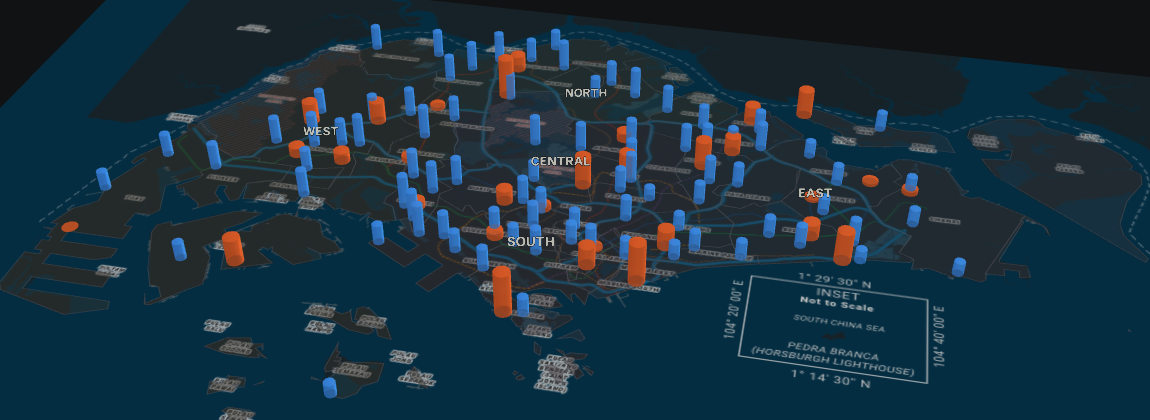
\includegraphics[width=0.66\textwidth]{figures/atlas.png}
\caption{The risk atlas. Blue columns are NEA rain gauges (share of working days with a 20\,mm rain hour). Orange columns are NEA heat stations (share of days reaching WBGT 32\,\textdegree C).}
\end{figure}

\textbf{The day simulator and the tariff desk.} Anyone can replay a real day, or set the readings by hand, and see what every hawker centre would be paid. A day with PSI 230, a 40\,mm rain hour and 3 hot hours takes 68\% of a cooked food stall's sales. On Tier 1 it would pay each stall \sgd 23.79, or \sgd 138,862 across all 5,837 stalls. Income's underwriters use the tariff desk to change any weight, band, tier, limit or premium share. They see the new prices at once, and save the change as a new version.

% ---------------------------------------------------------------- 8
\section{Distribution, pilot and our ask}\label{sec:pilot}

\subsection{Why should Income lead this?}

\begin{itemize}[leftmargin=1.2em]
  \item We found no product on sale in Singapore that pays hawkers or small shops for sales lost to haze, rain or heat when nothing is damaged. Swiss Re's HazeShield covers haze only, for larger businesses.\cite{ps}
  \item It builds on Income's own Droplet experience with parametric cover.
  \item It fills the gap SmartBiz 360 leaves when nothing is damaged.
  \item It fits Income's mission to serve people whose needs traditional insurance does not meet,\cite{income-agm} and it gives Income live data on its climate exposure.
\end{itemize}

\subsection{How would the pilot run?}

{\small
\begin{xltabular}{\textwidth}{|K{2.6cm}|Y|}
\hline
Months 0 to 3 & \textbf{What happens:} an actuarial review of the tariff and the premium shares, a reinsurance quote, NEA's check of heat stations S142 and S128, an agreement with one hawker association, a short survey of what stallholders will pay for each tier, and a PDPA review.\newline \textbf{How we know it works:} Income approves the tariff. \\
\hline
Months 3 to 9 & \textbf{What happens:} a live pilot with about 300 stalls and real PayNow payouts.\newline \textbf{How we know it works:} every payout is made on the day, 90\% of customers pass the say-it-back check, and disputes and renewals are tracked. \\
\hline
Months 9 to 12 & \textbf{What happens:} we tune the weights with real sales data from pilot stalls, and add market stalls and shops.\newline \textbf{How we know it works:} payouts come close to each tier's payout share (55\% to 70\%), and stallholders renew. \\
\hline
Year 2 & \textbf{What happens:} Payung is offered with every SmartBiz 360 and Stallholder Insurance sale, then to platform workers.\newline \textbf{How we know it works:} uptake and the claims ratio, by segment. \\
\hline
\end{xltabular}}

\subsection{What are the limits?}

\begin{itemize}[leftmargin=1.2em]
  \item Heat data in NEA's open feed starts only in 2025, so heat prices carry extra uncertainty for now.
  \item Heat stations S142 and S128 are on hold until NEA confirms their readings. If NEA confirms them, the stalls near them will cost more.
  \item The premium shares, and the split of running costs into management and selling, are our assumptions until Income gives its own cost figures.
  \item Flood is priced at zero until PUB shares its water level history, which we have requested.
  \item Lockdowns are priced at 2 days a year, one 40-day lockdown every 20 years, and the severe haze payout at a 5.5\% chance a year. Both are team assumptions until Income gives its view.
  \item The reinsurance structure is open. The 6\% share is our assumption, not a quote.
  \item We have no survey of what stallholders will pay. Tier 1 for cooked food is more than a few dollars a week, and the pilot must show whether stallholders buy it.
  \item Daily sales are declared by the customer. The platform does not check them against records yet.
  \item Most tiers fail the self-insure test on weather alone, and shop products fail it everywhere (Section \ref{sec:value}). The commission and the lockdown price are open decisions.
  \item The values marked ``Assumption'' in Appendix \ref{app:params} are starting values. They will be agreed with Income's actuaries and checked against real sales data in the pilot.
\end{itemize}

\begin{tcolorbox}[colback=soft,colframe=accent,boxrule=0.6pt,arc=2pt,left=8pt,right=8pt,top=6pt,bottom=6pt]
\textbf{Our ask.} A six-month pilot with Income: about 300 stalls through one hawker association, real PayNow payouts, and a monthly report on payout speed, understanding, disputes and renewal. In an average year, a pilot book of 300 Tier 1 stalls earns Income about \biz{0.10}{300} after reinsurance. The platform, the pricing engine and the replayed history (haze from 2014, rain from 2016) are ready today.
\end{tcolorbox}

% ---------------------------------------------------------------- Appendix
\clearpage
\appendix
\renewcommand{\thesection}{\Alph{section}}
\section{Every value we use, and where it comes from}\label{app:params}

These are the values in the platform's current tariff. Each one can be changed in the tariff desk, and every change is saved as a new version. Each entry says what the value is, how it is used, and where it comes from:

\begin{itemize}[leftmargin=1.2em]
  \item \measured\ The value comes from public data.
  \item \assumed\ A starting value, still to be set with Income's actuaries and pilot sales data.
\end{itemize}

\subsection{What triggers a payout}

{\small
\begin{xltabular}{\textwidth}{|K{3.4cm}|Y|}
\hline
Haze reading & The highest 24-hour PSI of the day in the stall's region, one of NEA's five. It is matched to a severity step.\newline \measured\ NEA historical 24-hour PSI from Apr 2014, and NEA PSI on data.gov.sg from 9 Mar 2016 to 7 Nov 2026.\cite{team-data} \\
\hline
Haze steps & PSI 101, 201 and 301 start the three payout steps.\newline \measured\ These are NEA's own unhealthy, very unhealthy and hazardous bands. \\
\hline
Rain reading & The wettest hour between 7am and 7pm, in mm. We take the middle value of the 3 gauges nearest the stall.\newline \measured\ NEA rainfall on data.gov.sg, Dec 2016 to 8 Nov 2026.\cite{team-data} \\
\hline
Rain steps & 20, 30 and 50\,mm in an hour start the three payout steps.\newline \assumed \\
\hline
Heat reading & The number of hours between 7am and 7pm when WBGT at the nearest station is 32\,\textdegree C or more.\newline \measured\ NEA WBGT on data.gov.sg, Jan 2025 to Nov 2026. The 32\,\textdegree C level is MOM's rest-break level.\cite{team-data,mom} \\
\hline
Heat steps & 2, 4 and 6 hours start the three payout steps.\newline \assumed \\
\hline
Severity at each step & 30\%, 60\% and 100\%. This is Step 1 of the payout.\newline \assumed \\
\hline
Flood & A PUB flood alert during trading hours counts as a full loss. It is priced at 0 days a year for now.\newline \assumed\ Until PUB shares its flood history, which we have requested. \\
\hline
Lockdown or closure order & A government order that closes the business counts as a full day lost, for every product. It is priced at 2 days a year: one 40-day lockdown or closure order every 20 years.\newline \assumed\ No history. A team assumption until Income gives its view. \\
\hline
\end{xltabular}}

\subsection{How much of the day is lost}

{\small
\begin{xltabular}{\textwidth}{|K{3.4cm}|Y|}
\hline
Hazard weight & The share of sales lost at full severity: haze 0.8, rain 0.5, heat 0.4, flood 0.8, closure 1.0. This is Step 2 of the payout.\newline \assumed\ The haze weight is in line with the 20\% to 60\% falls stalls reported in October 2026.\cite{st-haze} \\
\hline
Gross margin & The profit on each sale after paying for the goods: 0.67 for cooked food, 0.32 for every other product.\newline \measured\ SingStat Annual Survey of Services 2024. Food and beverage outlets spend 32.9\% of revenue on goods, and retail shops 68.0\%.\cite{singstat} \\
\hline
Shelf life & How many days the stock lasts: cooked food 0.5, fresh produce 3, flowers 5, packaged food 180, general goods 365.\newline \assumed \\
\hline
Restock interval & How often the stall buys new stock, in days: cooked food 1, fresh produce 1, flowers 3, packaged food 7, general goods 30. The spoiled share is restock days divided by shelf life, at most 1.\newline \assumed \\
\hline
Demand lost & How much of a bad day's demand the product loses: cooked food 1.0, fresh produce 0.9, flowers 0.8, packaged food 0.6, general goods 0.5.\newline \assumed \\
\hline
Sales made up later & The share of lost sales that come back on later days, and so are not paid: 0 for cooked food, 0.5 for everything else.\newline \assumed \\
\hline
Product share & The result of the rows above: cooked food 1.00, fresh produce 0.35, flowers 0.45, packaged food and general goods 0.11. It multiplies every hazard's loss.\newline Calculated as: demand lost $\times$ [ margin $\times$ (1 $-$ sales made up later) $+$ spoiled share $\times$ (1 $-$ margin) ]. \\
\hline
\end{xltabular}}

\subsection{Location}

{\small
\begin{xltabular}{\textwidth}{|K{3.4cm}|Y|}
\hline
Stall location & The stall's hawker centre or postal code, turned into a point on the map. It is used to find the nearest stations.\newline \measured\ NEA Hawker Centres dataset.\cite{nea-hawker} \\
\hline
Region & The nearest of the five region points that NEA publishes with the PSI. It sets the haze reading and the region average.\newline \measured\ NEA PSI data on data.gov.sg. \\
\hline
Stations read & Haze uses the region; rain uses the middle of the 3 nearest gauges; heat uses the nearest station. A station that did not report that day is skipped, and the next nearest is read. The price replays every day through the same rule as the payout.\newline A design choice, following the lesson from Jakarta's single-gauge flood card. \\
\hline
Stations on hold & Heat stations S142 and S128 are skipped, for the price, the payout, the live score and every replay, as if they had not reported. S142 recorded 120 heat trigger days in 2026 and S128 recorded 50, against about 7 at a typical station.\newline \assumed\ Until NEA confirms the readings. \\
\hline
History used & PSI from 1 Apr 2014 to 7 Nov 2026 (NEA historical 24-hour PSI before the live feed starts on 9 Mar 2016), rain from Dec 2016 to 8 Nov 2026, and WBGT from Jan 2025 to Nov 2026.\newline \measured\ NEA on data.gov.sg.\cite{team-data} \\
\hline
Years without a feed & In a year before a hazard's feed started (rain before Dec 2016, heat before 2025), that hazard adds its average yearly loss-days from the years it was recorded. A part year is scaled up to a full year.\newline A pricing rule, so that every year counts every hazard. \\
\hline
\end{xltabular}}

\subsection{Price}

{\small
\begin{xltabular}{\textwidth}{|K{3.4cm}|Y|}
\hline
Tiers & \sgd 35, 195, 630 or 1,355 a day. Payout = day's loss $\times$ daily amount.\newline A product design choice, set by the team on 15 Nov 2026, to be agreed with Income. \\
\hline
Daily sales and the suggested tier & The business's normal sales on a weekday, \sgd 20 to \sgd 50,000, given at sign-up. A day with no sales costs those sales times the product share. The suggested tier is the biggest whose daily amount is at or below that; bigger tiers are not offered, and below \sgd 35 no tier is. Without the sales, every tier the place allows is shown and none is suggested. Rent is shown for information only.\newline A design choice by the team lead, 16 Nov 2026, so that cover never pays more than the loss (insurable interest). \\
\hline
Yearly limit & 45 full days in any 365 days, in every tier: \sgd 1,575, 8,775, 28,350 or 60,975. A 40-day lockdown is paid in full. The limit sits above a cooked food stall's worst replayed year at every centre (14.9 full days, 2026) and above a 2015-like weather year, with an average year of rain and heat (at most 18.9 full days, at Jurong West Street 52).\newline A product design choice, to be agreed with Income. \\
\hline
Waiting period & 30 days from the start of cover, and again for the whole cover after a move up a tier. A move down keeps the start date.\newline A design choice, so nobody buys or moves up only when a bad day is forecast. \\
\hline
Severe haze payout & An option on any tier. 40 or more days with the region's 24-hour PSI at 101 or more in a policy year pays 25 times the daily amount, once. Its yearly price is a tenth of that payout, GST included. Not sold from May to October. 30-day wait.\newline \assumed\ Priced as a 5.5\% chance a year, about 1 year in 18, with 60\% of the price paid out. Since Apr 2014 only 2015 reached 40 days, in 3 of the 5 regions.\cite{team-data} \\
\hline
Expected paid days & The average over the replayed years of min(that year's loss-days, the yearly limit), at the customer's place and for the chosen tier.\newline Calculated from the history above, with the payout rule. \\
\hline
Payout share & Expected payouts as a share of premium without GST: 55\%, 60\%, 65\% or 70\%, by tier. Premium without GST = expected paid days $\times$ daily amount $\div$ payout share.\newline \assumed\ Higher tiers spend a smaller share on fixed costs. \\
\hline
Reinsurance & 6\% of premium without GST in every tier, for haze and lockdown years.\newline \assumed\ The 10\% rare event load on a 60\% payout share. The structure (kept in-house, an excess layer or a share ceded) is still open. To be set with Income's reinsurance quote. \\
\hline
Management expenses & 12\%, 10\%, 8\% or 7\% of premium without GST, by tier.\newline \assumed\ Until Income gives its figure. \\
\hline
Selling and distribution & 17\%, 15\%, 13\% or 10\% of premium without GST, by tier.\newline \assumed\ Until Income gives its figure. Running costs of 17\% to 29\% are lower than the industry's 39.0\% and Income's 35.5\%,\cite{mas} because there is no claims handling. \\
\hline
Profit and risk margin & 10\%, 9\%, 8\% or 7\% of premium without GST, by tier.\newline \assumed\ The 15\% uncertainty load on a 60\% payout share, in line with ILO and World Bank practice.\cite{ilo,worldbank} \\
\hline
Not offered at a place & A tier whose yearly price is more than half its yearly limit is not offered at that place. The quote shows ``not offered here'' with the reason, and the platform refuses to sell it. No tier is referred to the underwriter for its price.\newline A design choice, so no customer buys cover that pays back less than twice its price in the worst year. No tier is above it at the final prices. \\
\hline
GST & 9\%, added on top and passed to IRAS.\newline \measured\ IRAS.\cite{iras} \\
\hline
Months, weeks and days a year & 12, 52 and 365. Monthly price = yearly price $\div$ 12. Weekly price = yearly price $\div$ 52. Price per day = yearly price $\div$ 365. The premium is collected weekly. \\
\hline
Older tariffs & A saved tariff without premium shares is priced with the original loads: 15\% uncertainty and 10\% rare event on expected payouts, then running costs of 25\%. For Tier 2 these give the same price as the shares above. \\
\hline
\end{xltabular}}

\subsection{Data sources}

{\small
\begin{xltabular}{\textwidth}{|K{4.2cm}|Y|}
\hline
NEA 24-hour PSI & Haze readings by region, and the five region points. Open, through the data.gov.sg API. The historical PSI from Apr 2014 is also open on data.gov.sg. \\
\hline
NEA rainfall & Rain every 5 minutes at every gauge, and gauge locations. Open, through the data.gov.sg API. \\
\hline
NEA WBGT & Heat stress readings and station locations. Open, through the data.gov.sg API. \\
\hline
NEA Hawker Centres & 103 centres and 5,837 cooked food stalls, with locations. Open, on data.gov.sg. \\
\hline
SingStat Annual Survey of Services & Gross margins for food and beverage outlets and for retail shops. Open, on data.gov.sg. \\
\hline
MAS insurance returns & Claims and expense ratios for the industry and for Income. Open, on the MAS website. \\
\hline
MOM heat stress measures & The 32\,\textdegree C rest-break level. Open, on the MOM website. \\
\hline
PUB flood alerts and history & The flood trigger, and flood days for the price. Alerts are open; we have requested the history by email. \\
\hline
ECMWF forecasts via Open-Meteo & Early warnings, and the proposed sales pause, only. Never payouts. Open API. \\
\hline
MSE and MOM parliamentary replies and speeches & Hawker income, stall rent, charges and operating costs, and platform workers' earnings, for the affordability check. Open, on the MSE and MOM websites. \\
\hline
\end{xltabular}}

% ---------------------------------------------------------------- References
\renewcommand{\refname}{\large References}
{\footnotesize\raggedright
\setlength{\bibsep}{1pt}
\begin{thebibliography}{99}
\bibitem{ps} Income Insurance, \emph{SIH 2026 Industry Track Problem Statements}, FinTech/InsurTech, Singapore-India Hackathon 2026.
\bibitem{mse-hawker} Ministry of Sustainability and the Environment, written reply to parliamentary question on insurance for hawkers, 4 Aug 2026.
\bibitem{koh-hawker} Ministry of Sustainability and the Environment, response to the motion on hawker culture by Senior Minister of State Dr Koh Poh Koon, 13 Nov 2024, paragraphs 24 to 26, 39 and 62.
\bibitem{mse-rent} Ministry of Sustainability and the Environment, written reply to parliamentary question on average monthly costs of cooked food stalls, 8 Sep 2026 (2025 figures).
\bibitem{nea-hawker} National Environment Agency, Hawker Centres dataset (existing centres and cooked food stalls), data.gov.sg, accessed Nov 2026.
\bibitem{st-haze} The Straits Times via Asia News Network, ``Singapore's F\&B businesses struggle as haze conditions worsen'', 19 Oct 2026.
\bibitem{stb} TTG Asia, ``Visitor arrivals to Singapore increase as tourism receipts grow'', 3 Feb 2026, citing the Singapore Tourism Board.
\bibitem{heatsafe} NUS Yong Loo Lin School of Medicine, Project HeatSafe press release, 18 Mar 2024.
\bibitem{ntu-haze} E.~Quah (NTU) and E.~Or (SUSS), ``Haze in 2026 estimated to cost Singapore \sgd 2.32b'', NTU School of Social Sciences, 8 Nov 2026.
\bibitem{team-data} Payung team analysis of NEA open data on data.gov.sg (24-hour PSI from Apr 2014, rainfall from Dec 2016, WBGT from Jan 2025, to 8 Nov 2026), with ECMWF forecasts via Open-Meteo; scripts in the team's GitHub repository.
\bibitem{mom} Ministry of Manpower, heat stress measures for outdoor work.
\bibitem{mss-2025} Meteorological Service Singapore, Annual Climate Assessment 2025, 23 Mar 2026.
\bibitem{v3} Meteorological Service Singapore and Ministry of Sustainability and the Environment, joint release on Singapore's Third National Climate Change Study (V3), 5 Jan 2024.
\bibitem{nccs} National Climate Change Secretariat, Coastal Protection.
\bibitem{vamei} C.-P.~Chang, C.-H.~Liu and H.-C.~Kuo, ``Typhoon Vamei: an equatorial tropical cyclone formation'', \emph{Geophysical Research Letters} 30(3), 2003.
\bibitem{fudai} Associated Press, ``Once-belittled floodgate saved Japanese town'', 15 May 2011.
\bibitem{chennai} Swiss Re sigma estimates for the 2015 Chennai floods, as reported by Business Standard, 30 Mar 2016.
\bibitem{mercy} Mercy Corps and Okapi Research, \emph{Transforming Chennai: building micro, small and medium enterprise resilience to water-related risks}.
\bibitem{income-qa} Income Insurance product lead, private mentoring session with the team, 15 Nov 2026, as recorded in the team's notes.
\bibitem{mom-platform} Ministry of Manpower, speech by Senior Minister of State Dr Koh Poh Koon at the second reading of the Platform Workers Bill, 9 Sep 2024.
\bibitem{income-stall} Income Insurance, Stallholder Insurance product brochure, rates from 1 Jul 2024.
\bibitem{marsh} Marsh Risk Consulting, \emph{Gross Profit (UK) vs.\ Gross Earnings (US)}, 2012.
\bibitem{zurich} Zurich UK, ``Deterioration of stock cover explained''.
\bibitem{singstat} Department of Statistics Singapore, Annual Survey of Services 2024, data.gov.sg datasets d\_38d62de582eb7ee2c58d1bba4cd4132d and d\_4eb10d0ef99e56c2336c37d78b10c6bc.
\bibitem{worldbank} World Bank, \emph{Weather Index Insurance for Agriculture: Guidance for Development Practitioners}, 2011, Box 5.3.
\bibitem{mas} Monetary Authority of Singapore, Insurance Statistics 2021 to 2025 and Income Insurance Limited returns (I585C).
\bibitem{grab} Grab, free insurance for driver-partners, grab.com/sg/driver/finance/insurance.
\bibitem{mas-fd} Monetary Authority of Singapore, \emph{Guidelines on Fair Dealing} (FSG-G04), 30 May 2024.
\bibitem{ilo} P.~Wrede and C.~Phily, \emph{Pricing for Microinsurance: A Technical Guide}, ILO Microinsurance Innovation Facility, 2012, p.~44.
\bibitem{income-agm} Income Insurance, minutes of the Annual General Meeting, 25 May 2026.
\bibitem{iras} Inland Revenue Authority of Singapore, GST rate of 9\% from 1 Jan 2024.
\bibitem{werner} G.~Werner and C.~Modlin, \emph{Basic Ratemaking}, 5th ed., Casualty Actuarial Society, 2016, chapters 11 and 12.
\end{thebibliography}
}

\end{document}
